\documentclass{beamer}
\usepackage[utf8]{inputenc}
\usepackage[UKenglish]{babel}
\usepackage[UKenglish]{isodate}
\usepackage{amsmath}
\usepackage{mathtools}
\usepackage{tikz}
\usepackage{complexity}
\usepackage[style=authoryear]{biblatex}
\usepackage{forest}
\usepackage{soul}
\usepackage{csquotes}
\usepackage{pifont}

\usetikzlibrary{shapes}
\usetikzlibrary{positioning}
\usetikzlibrary{overlay-beamer-styles}
\usetikzlibrary{shapes.callouts}
\usetikzlibrary{cd}
\usetikzlibrary{calc}
\usetikzlibrary{backgrounds}
\usetikzlibrary{fit}
\usetikzlibrary{decorations.pathreplacing}

\newcommand\blfootnote[1]{%
  \begingroup
  \renewcommand\thefootnote{}\footnote{#1}%
  \addtocounter{footnote}{-1}%
  \endgroup
}

\renewcommand<>{\hl}[1]{\only#2{\beameroriginal{\hl}}{#1}}
\makeatletter
\newcommand\SoulColor{%
  \let\set@color\beamerorig@set@color
  \let\reset@color\beamerorig@reset@color}
\makeatother
\SoulColor

\beamertemplatenavigationsymbolsempty
\usetheme{metropolis}
\setbeamercolor{background canvas}{bg=white}

\addbibresource{talk.bib}

\definecolor{color1}{HTML}{1B9E77}
\definecolor{color2}{HTML}{7570b3}
\definecolor{color3}{HTML}{a6761d}
\definecolor{forestgreen}{HTML}{009B55}

\DeclareMathOperator{\GDR}{\textsc{GDR}}
\DeclareMathOperator{\CR}{\textsc{CR}}
\DeclareMathOperator{\Reff}{\textsc{Ref}}

\colorlet{redish}{color2!25}
\colorlet{greenish}{color1!25}
\colorlet{blueish}{color3!25}
\sethlcolor{redish}
\setstcolor{black}

\tikzset{
  inner/.style={
    ellipse,
    draw,
  },
  inner on/.style={alt=#1{inner}{}},
  leaf/.style={
    rectangle,
    draw,
    fill=gray!25,
  },
  leaf on/.style={alt=#1{leaf}{}},
  invisible/.style={opacity=0,text opacity=0},
  visible on/.style={alt=#1{}{invisible}},
  alt/.code args={<#1>#2#3}{%
    \alt<#1>{\pgfkeysalso{#2}}{\pgfkeysalso{#3}} % \pgfkeysalso doesn't change the path
  },
}

\forestset{
sn edges/.style={for tree={edge={-Latex}}},
  visible on/.style={
    for tree={
      /tikz/visible on={#1},
      edge+={/tikz/visible on={#1}}}}
}

\newcommand{\cmark}{\ding{51}}%

\newcommand{\xx}{\textcolor{color1}{x}}
\newcommand{\yy}{\textcolor{color3}{y}}
\newcommand{\pP}{\texttt{P}}
\newcommand{\qQ}{\texttt{Q}}
\newcommand{\dDelta}{\textcolor{color2}{\Delta}}

\newcommand{\pone}{\textcolor{color1}{\pP(1)}}
\newcommand{\ptwo}{\textcolor{color1}{\pP(2)}}
\newcommand{\qone}{\textcolor{color2}{\qQ(1)}}
\newcommand{\qtwo}{\textcolor{color2}{\qQ(2)}}
\newcommand{\pqone}{\textcolor{color3}{\pP(1)}, \textcolor{color3}{\qQ(1)}}
\newcommand{\pqtwo}{\textcolor{color3}{\pP(2)}, \textcolor{color3}{\qQ(2)}}

\newcommand{\WMC}{\textup{WMC}}
\newcommand{\WMI}{\textup{WMI}}
\newcommand{\WFOMI}{\textup{WFOMI}}
\newcommand{\AMC}{\textup{AMC}}
\newcommand{\pbp}{\textup{PBP}}
\newcommand{\SPPP}{\textup{SP}}

% 15 min (8 slides, currently have 7) introduction
% 25 min (13 slides, currently have 10) presentation
% 5 min (3 slides, currently have 1) summary
% make sure there's a clear and coherent storyline

\author{Paulius Dilkas \\ \vspace{1cm} \tiny{Joint work with Vaishak Belle (Univeristy of Edinburgh, UK)}}
\title{Synthesising Recursive Functions for\\ First-Order Model Counting}
\institute{National University of Singapore, Singapore}
\date{18th April 2023}
% TODO: unify the use of colours, maybe replace red!50 with one of the main colours
% TODO: how do we capitalise titles of \block?
% TODO: make sure I'm using the 'forest' package whenever possible

\begin{document}
\addtobeamertemplate{block begin}{\setlength\abovedisplayskip{0pt}}

\begin{frame}[noframenumbering,plain]
  \tikz[remember picture,overlay]{
    \node at ([yshift=20pt,xshift=-20pt]current page.south)
    {
\includegraphics[height=40pt]{nus.jpg}};
    \node at ([yshift=25pt,xshift=30pt]current page.south)
    {
\includegraphics[height=40pt]{inf.png}};
    \node at ([yshift=25pt,xshift=75pt]current page.south)
    {
\includegraphics[height=40pt]{ecr.jpg}};
    \node at ([yshift=20pt,xshift=140pt]current page.south)
    {
\includegraphics[height=20pt]{epsrc.png}};
  }
  \titlepage
\end{frame}

\begin{frame}{What Computers Can and Cannot Do}
  \begin{tikzpicture}[remember picture,overlay]
    \node[right=0.7cm] at (current page.west) (stickman) {
\includegraphics[height=0.5\textheight]{stickman.png}};
    \node<-4>[left,shift=({0, -2})] at (current page.east) (computer) {
\includegraphics[height=0.5\textheight]{happy_computer}};
    \node<2>[ellipse callout, draw, right=0cm, callout relative pointer={(-1, -0.5)}] at (stickman.north east) {$\int_{-\infty}^{\infty} e^{-t^{2}}\,\mathrm{d}t$};
    \node<2>[ellipse callout, draw, left=-0.5cm, below=0.5cm] at (computer.north west) {$\sqrt{\pi}$};
    \node<3>[ellipse callout, draw, right=0cm, callout relative pointer={(-1, -0.15)},text width=5cm] at (stickman.north east) {Produce a schedule for the nurses at the local hospital.};
    \node<3>[ellipse callout, draw, below=0.5cm, shift=({-0.5,0}), callout relative pointer={(0.5, -0.25)}] at (computer.north west) {
\includegraphics[width=0.1\textwidth]{schedule}};
    \node<4>[ellipse callout, draw, right=0cm, callout relative pointer={(-1, -0.15)},text width=6cm] at (stickman.north east) {Paint a baroque oil painting of a \alert{raccoon queen wearing a crown}.};
    \node<4>[ellipse callout, draw, below=0cm, shift=({-1.5,1}), callout relative pointer={(0.4, -0.2)}] at (computer.north west) {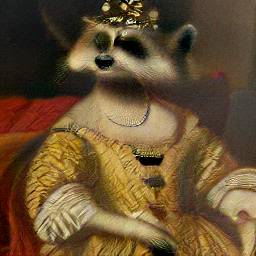
\includegraphics[width=0.25\textwidth]{dalle.png}};
    \node<5>[ellipse callout, draw, right=0cm, callout relative pointer={(-1, -0.15)}, text width=5cm] at (stickman.north east) {If I shuffle a deck of \alert{$n$} cards, how many possible outcomes are there?};
    \node<5>[left,shift=({-1, -1})] at (current page.east) (computer2) {
\includegraphics[height=0.5\textheight]{overheating_computer}\blfootnote{Terms and conditions apply.}};
    \node[shift=({1.3, 0.1})] at (current page.south west) {\tiny \textcolor{lightgray}{Vector art by Vecteezy.com}};
  \end{tikzpicture}
\end{frame}

\begin{frame}{Who Cares About Counting?}
  \begin{columns}
    \begin{column}{0.5\textwidth}
      \pause
      \begin{block}{\alert{Probabilistic Programming}}
        \centering
        
\includegraphics[width=\textwidth]{programming.png}
      \end{block}
      \pause
      \begin{block}{\alert{Neuro-symbolic AI}}
        \centering
        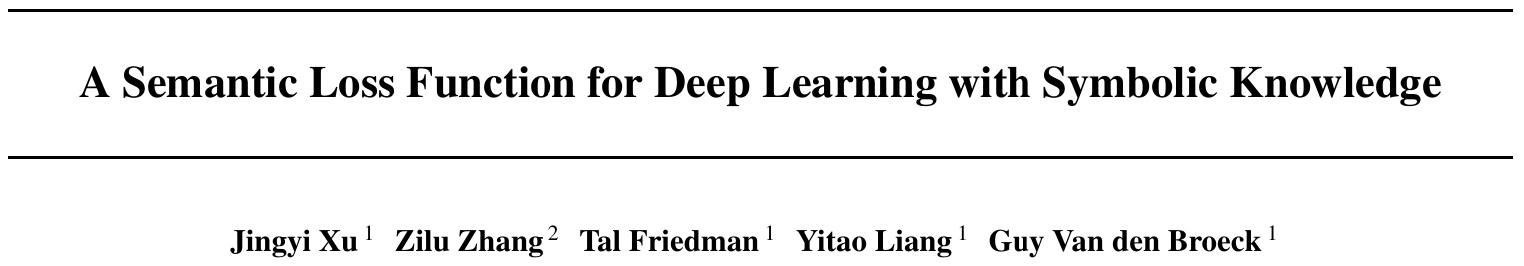
\includegraphics[width=\textwidth]{neurosymbolic.png}
      \end{block}
      \pause
      \begin{block}{\alert{Natural Language Processing}}
        \centering
        
\includegraphics[width=\textwidth]{knowledge.png}
      \end{block}
      \pause
    \end{column}
    \begin{column}{0.5\textwidth}
      \begin{block}{\alert{Robotics}}
        \centering
        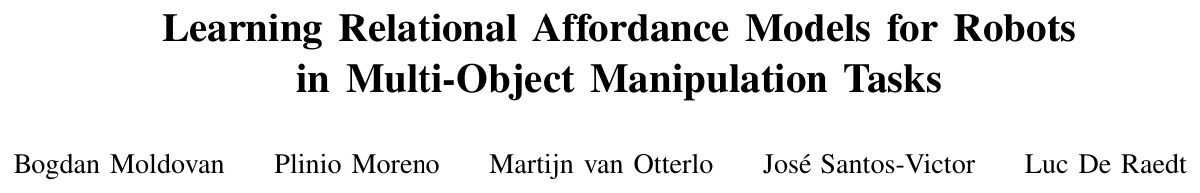
\includegraphics[width=\textwidth]{ICRA.png}
      \end{block}
      \pause
      \begin{block}{\alert{Bioinformatics}}
        \centering
        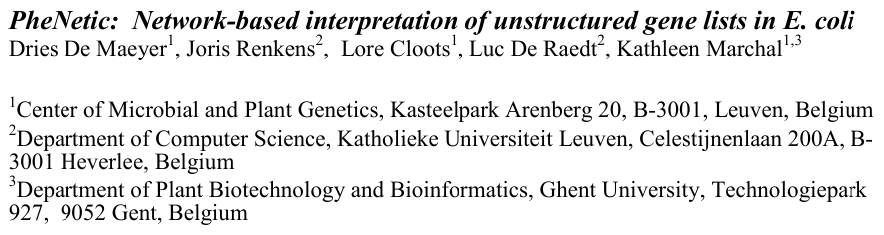
\includegraphics[width=\textwidth]{bio.png}
      \end{block}
      \pause
      \begin{block}{\alert{Combinatorics}}
        \centering
        
\includegraphics[width=\textwidth]{recurrence.png}
      \end{block}
    \end{column}
  \end{columns}
\end{frame}

\begin{frame}[fragile]{(Some of the) Many Ways to Count}
  \begin{center}
    \begin{tikzcd}[remember picture]
      |[alias=WMI,visible on=<7->]|\WMI{} & |[visible on=<7->]|\WFOMI{} \\
      |[alias=WMC]|\#\SAT{}/\WMC{} \arrow[u,visible on=<7->] \ar[d,visible on=<8->] \ar[r,visible on=<5->] & |[visible on=<5->]|\textup{(W)\alert<9>{FOMC}} \arrow[u,visible on=<7->] \ar[d,visible on=<8->] \\
      |[alias=PBP,visible on=<8->]|\AMC{}, \pbp{} & |[alias=SP,visible on=<8->]|\SPPP{}
    \end{tikzcd}
  \end{center}
  \begin{tikzpicture}[overlay,remember picture]
    \begin{scope}[transform canvas={xshift=-3em}]
      \draw[->,draw=gray] ($(WMC)+(0,0.1)$)--($(WMI)+(0,0.5)$) node[midway,left,visible on=<7->] {\textcolor{gray}{$\sum \to \int$}};
      \draw[->,draw=gray] ($(WMC)-(0,0.1)$)--($(PBP)-(0,0.5)$) node[midway,left,visible on=<8->] {\textcolor{gray}{Generalising weights}};
    \end{scope}
    \begin{scope}[transform canvas={yshift=-2em}]
      \draw[->,draw=gray] ($(PBP)-(1,0)$)--($(SP)+(1,0)$) node[midway,below,visible on=<5->] {\textcolor{gray}{From propositional to first-order logic}};
    \end{scope}
  \end{tikzpicture}
  \vfill
    \begin{overprint}
      \onslide<1,2>
      \begin{block}{\#SAT~\textcolor{gray}{\parencite{DBLP:journals/tcs/Valiant79}}}
        \begin{itemize}
          \item Input formula: $\xx \lor \yy$
          \item Interpretations: $\emptyset$, $\{\, \xx \,\}$, $\{\, \yy \,\}$,
                $\{\, \xx, \yy \,\}$
          \item Models: $\{\, \xx \,\}$, $\{\, \yy \,\}$, $\{\, \xx, \yy \,\}$
          \item<2-> Answer (model count): 3
        \end{itemize}
      \end{block}
      \onslide<3,4>
      \begin{block}{Weighted Model Counting~\textcolor{gray}{\parencite{DBLP:journals/ai/ChaviraD08}}}
        \begin{itemize}
          \item Input formula: $\xx \lor \yy$
          \item Input weights: $\begin{aligned}[t]
                                  &w(\xx) = 0.3\text{, }w(\neg \xx) = 0.7,\\
                                  &w(\yy) = 0.2\text{, }w(\neg \yy) = 0.8
                                \end{aligned}$
          \item<4-> Answer (weighted model count):
                $w(\xx)w(\yy) + w(\xx)w(\neg \yy) + w(\neg \xx)w(\yy) = 0.44$
        \end{itemize}
      \end{block}
      \onslide<5,6>
      \begin{block}{(Weighted) (Symmetric) First-Order Model Counting\\
          \textcolor{gray}{\parencite{DBLP:conf/ijcai/BroeckTMDR11}}}
        \begin{itemize}
          \item Input formula: $\forall \xx \in \Delta\text{. }\pP(\xx)$
          \item Input weights: $w^{+}(\pP) = 0.3$, $w^{-}(\pP) = 0.7$
          \item Input domain size(s): $|\dDelta| = 2$
          \item<6-> Answer: ${(w^{+}(\pP))}^{|\dDelta|} = 0.09$
        \end{itemize}
      \end{block}
      \onslide<7>
      \begin{block}{Extensions to Continuous Domains}
        \begin{itemize}
          \item Weighted model integration
          \begin{itemize}
            \item \textcolor{gray}{\parencite{DBLP:conf/ijcai/BellePB15}}
          \end{itemize}
          \item Weighted first-order model integration
          \begin{itemize}
            \item \textcolor{gray}{\parencite{DBLP:conf/uai/FeldsteinB21}}
          \end{itemize}
        \end{itemize}
      \end{block}
      \onslide<8>
      \begin{block}{Generalisations of the weight function}
        \begin{itemize}
          \item Algebraic model counting
          \begin{itemize}
            \item \textcolor{gray}{\parencite{DBLP:journals/japll/KimmigBR17}}
            \item From $\mathbb{R}_{\ge 0}$ to commutative semirings
          \end{itemize}
          \item Pseudo-Boolean projection~\textcolor{gray}{\parencite{DBLP:conf/sat/DilkasB21}}
          \begin{itemize}
            \item Weights not necessarily on literals
          \end{itemize}
          \item Semiring programming~\textcolor{gray}{\parencite{DBLP:journals/ijar/BelleR20}}
        \end{itemize}
      \end{block}
    \end{overprint}
\end{frame}
% maybe mention #CSP and other non-SAT ways of counting (SMT?, counting paths in
% automata and directed graphs)

\begin{frame}{(Unweighted) First-Order Model Counting}
  \begin{itemize}
    \item Example formula: \\
          \alert{$\forall x \in \Delta\text{. } \pP(x) \lor \qQ(x)$}
    \item Let \alert{$\Delta \coloneqq \{\, 1, 2 \,\}$}
    \item Interpretations: all subsets of\\
          \alert{$\{\, \pP(1), \qQ(1), \pP(2), \qQ(2) \,\}$}
    \item<2-> Models:
    \[
      \begin{matrix}
        \{\, \pone, \ptwo \,\}, & \{\, \pone, \qtwo \,\}, & \{\, \pone, \pqtwo \,\},\\
        \{\, \qone, \ptwo \,\}, & \{\, \qone, \qtwo \,\}, & \{\, \qone, \pqtwo \,\},\\
        \{\, \pqone, \ptwo \,\}, & \{\, \pqone, \qtwo \,\}, & \{\, \pqone, \pqtwo \,\}\\
      \end{matrix}
    \]
  \end{itemize}
  \onslide<3->{
    \begin{block}{Intuition}
      \begin{itemize}
        \item Each 1-ary predicate is like a \alert{subset}
        \item For \alert{$n>1$}, each \alert{$n$}-ary predicate is like a
              \alert{relation}
        \item FOMC counts \alert{combinations of relations}
      \end{itemize}
    \end{block}
  }
  \begin{tikzpicture}[remember picture,overlay,visible on=<2->]
    \tikzset{shift={(current page.north east)}}
    \tikzset{shift={(-4, -2.9)}}
    \node[draw,circle,minimum size=3cm,label={135:$\pP$},fill=color1] (P) at (0,0) {};
    \node[draw,circle,minimum size=3cm,label={45:$\qQ$},fill=color2] (Q) at (1.8,0) {};
    \begin{scope}
      \clip (0,0) circle(1.5cm);
      \clip (1.8,0) circle(1.5cm);
      \fill[color3](0,0) circle(1.5cm);
    \end{scope}
    \draw (0,0) circle(1.5cm);
    \draw (1.8,0) circle(1.5cm);
  \end{tikzpicture}
\end{frame}

\begin{frame}{Approaches to FOMC}
  \begin{itemize}
    \item \alert{ForcLift}~\textcolor{gray}{\parencite{DBLP:conf/ijcai/BroeckTMDR11}}
    \begin{itemize}
      \item knowledge compilation to \alert{FO d-DNNF}
    \end{itemize}
    \item \alert{L2C}~\textcolor{gray}{\parencite{DBLP:conf/kr/KazemiP16}}
    \begin{itemize}
      \item knowledge compilation to \alert{C++} code
    \end{itemize}
    \item \alert{Alchemy}~\textcolor{gray}{\parencite{DBLP:journals/cacm/GogateD16}}
    \begin{itemize}
      \item \alert{DPLL}-style search
    \end{itemize}
    \item \alert{FastWFOMC}~\textcolor{gray}{\parencite{DBLP:conf/uai/BremenK21}}
    \begin{itemize}
      \item knowledge compilation to \alert{sd-DNNF}
    \end{itemize}
  \end{itemize}
  \pause
  \vfill
  \begin{block}{Our Contribution}
    \centering
    \begin{tikzpicture}[align=center,node distance=0.1cm]
      \node[label=below:{ForcLift}] (forclift) {\includegraphics[width=0.2\paperwidth]{forklift.png}};
      \node[right=of forclift] (plus) {\Huge$+$};
      \node[right=of plus,label=below:{Recursion}] (recursion) {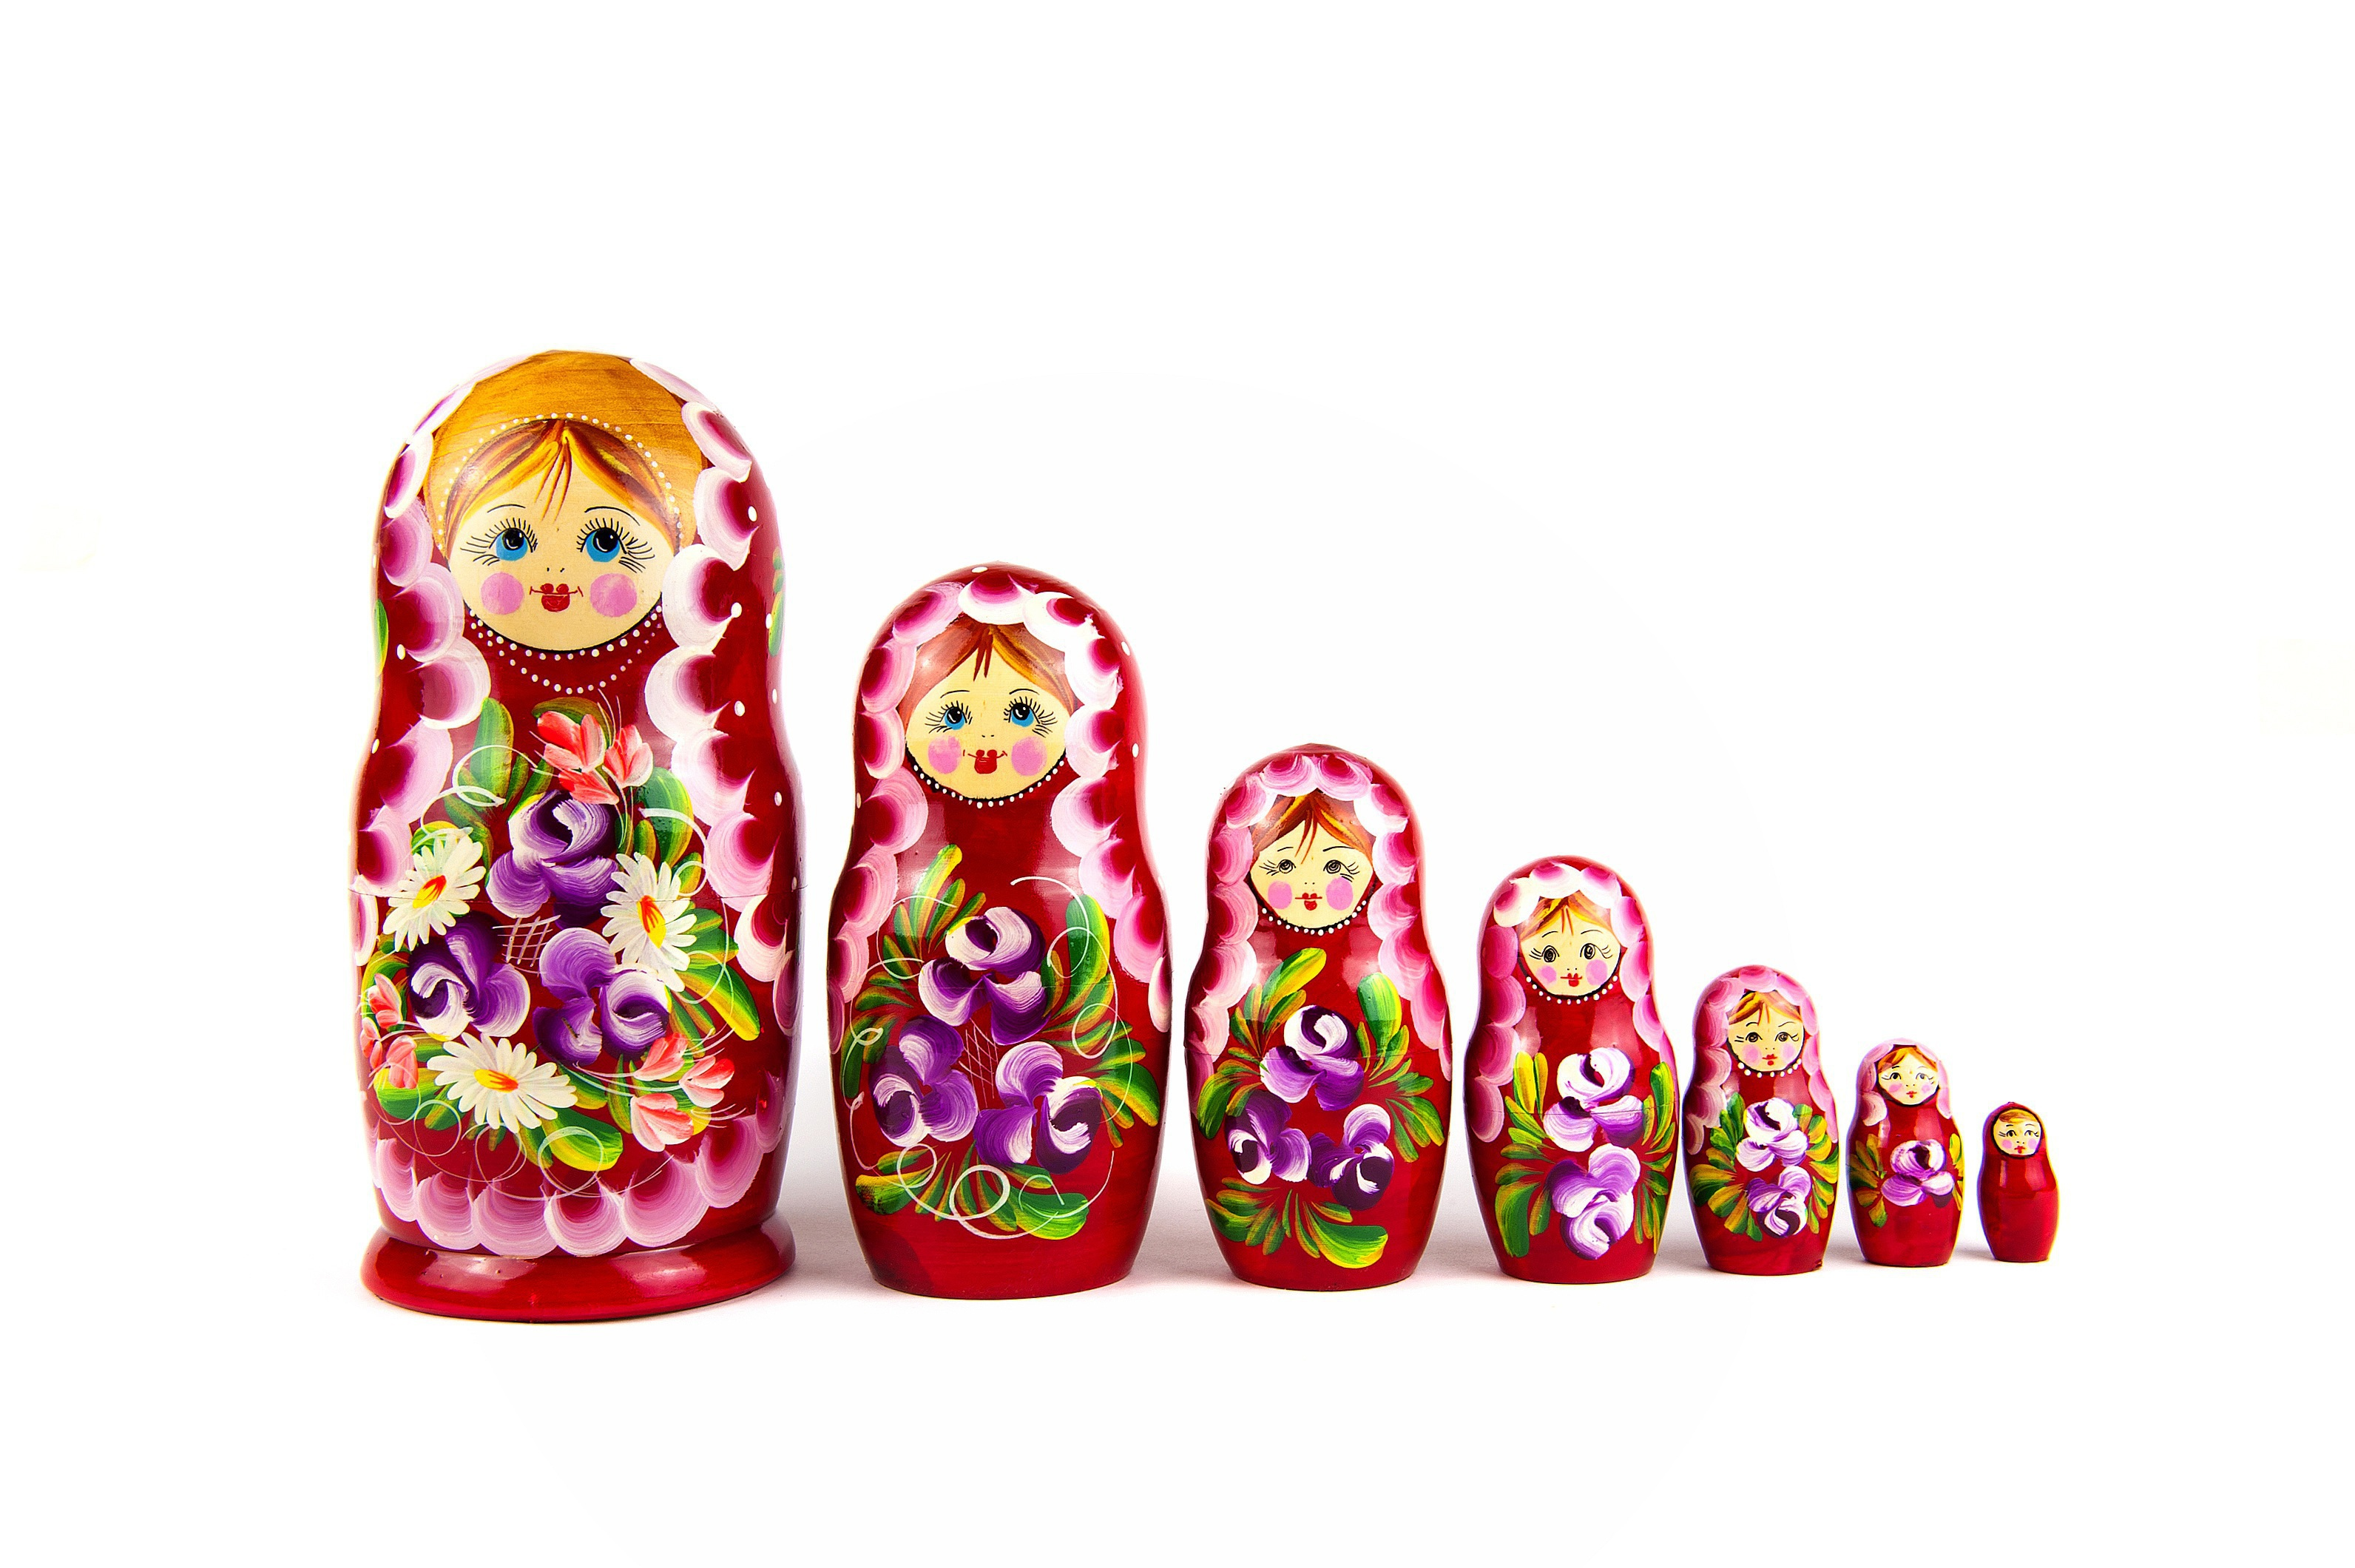
\includegraphics[width=0.2\paperwidth]{matryoshka.jpg}};
      \node[right=of recursion] (equal) {\Huge$=$};
      \node[right=of equal,label=below:{Crane}] (crane) {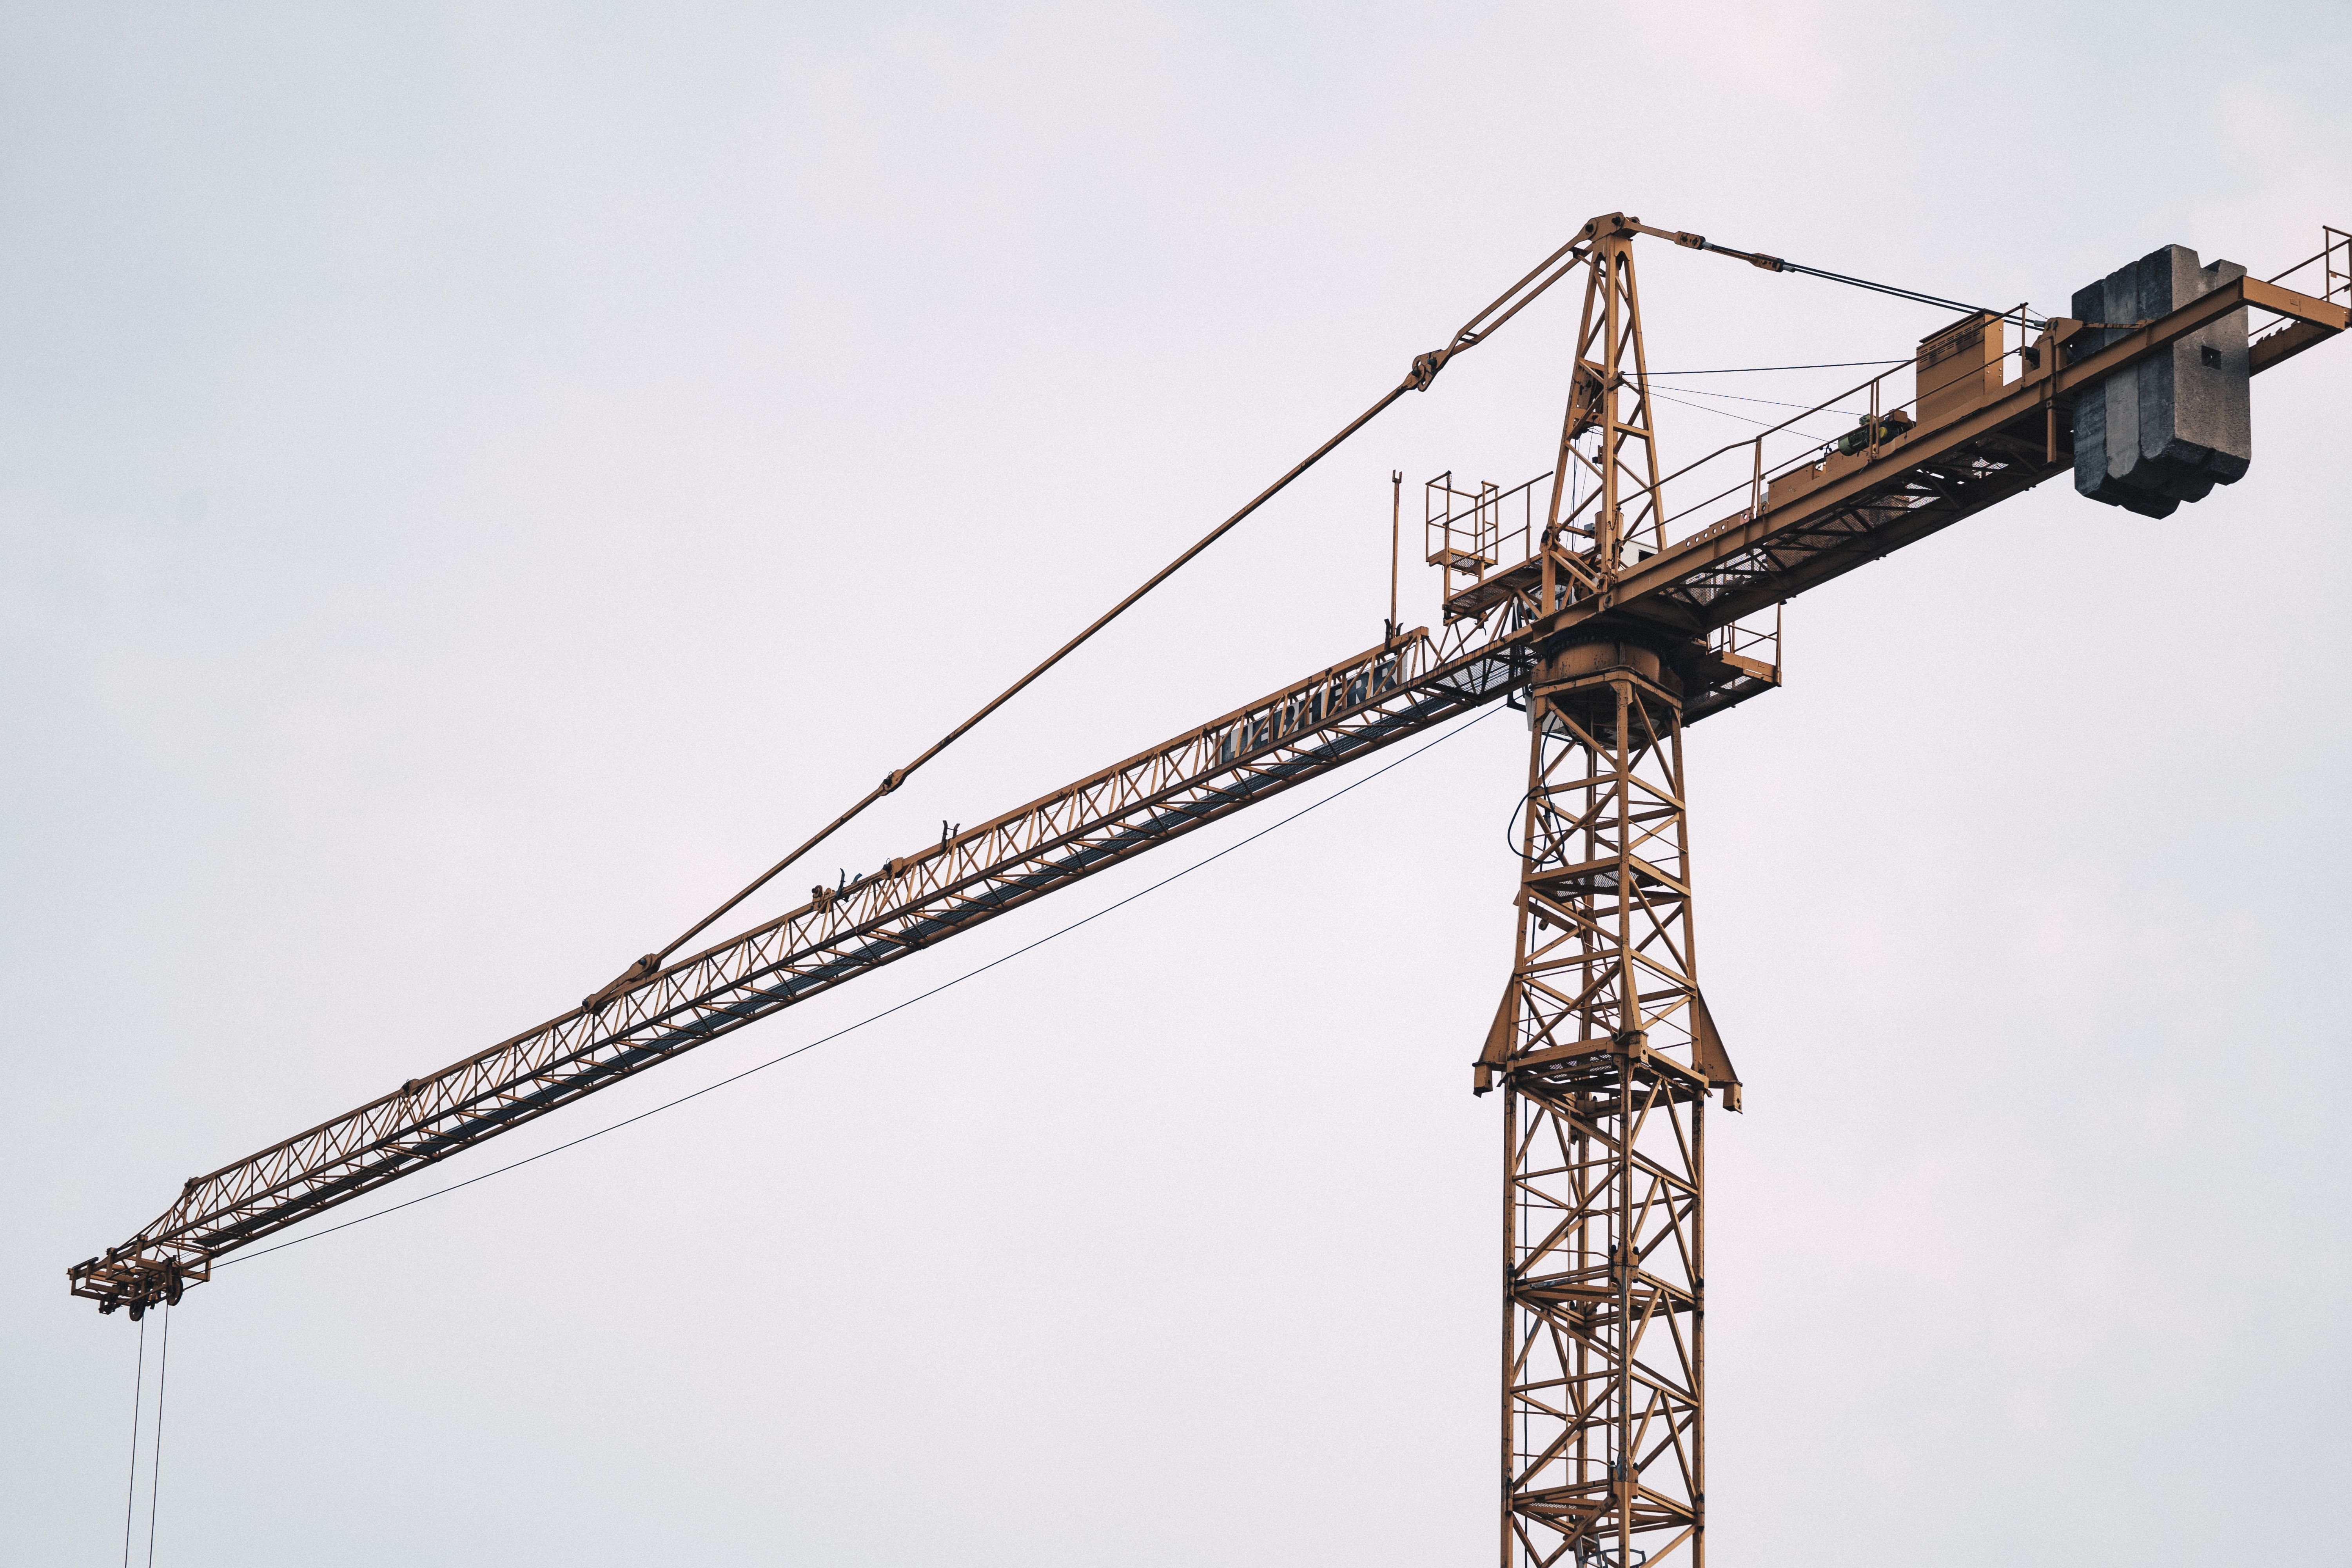
\includegraphics[width=0.2\paperwidth]{crane.jpg}};
    \end{tikzpicture}
  \end{block}
\end{frame}

\begin{frame}{ForcLift and First-Order Knowledge Compilation}
  \begin{minipage}[t][0.81\textheight][t]{\textwidth}
    \centering
    \begin{forest}
      for tree={s sep=10mm, sn edges}
      [\alt<3->{$\bigwedge_{c \in \Delta}$}{$\forall x \in \Delta\text{. } \pP(x) \lor \qQ(x)$},
      inner on=<3->,
      label={[visible on=<{13-14,19-}>]right:{\alert{\alt<15->{$3^{|\Delta|}$}{$\{\,\pP(c), \qQ(c)\,\}$}}}}
      [\alt<5->{$\lor$}{$\pP(c) \lor \qQ(c)$},
      name=lor,
      for tree={visible on=<3->},
      inner on=<5->,
      label={[visible on=<{12-14,18-}>]right:{\alert{\only<18->{$2 + 1 = 3$}\only<12-13>{\colorbox{white}{$\{\,\pP(c), \qQ(c)\,\}$}}\only<14>{\colorbox{redish}{$\{\,\pP(c), \qQ(c)\,\}$}}}}}
      [\alt<7->{$\land$}{$\begin{aligned}\qQ(c)\\ \pP(c) \lor \qQ(c)\end{aligned}$},
      name=and,
      for tree={visible on=<5->},
      inner on=<7->,
      label={[visible on=<{11-14,17-}>]left:{\alert{\only<17->{$2 \times 1 = 2$}\only<11-13>{\colorbox{white}{$\{\,\qQ(c)\,\}$}}\only<14>{\colorbox{redish}{$\{\,\qQ(c)\,\}$}}}}}
      [\alt<15->{$\pP(c) \lor \neg \pP(c)$}{$\qQ(c)$},
      name=smoothing,
      for tree={visible on=<7->},
      rectangle,
      draw,
      fill=gray!25,
      label={[visible on=<16->]below:{\alert{2}}}]
      [\alt<15->{$\land$}{$\top$},
      for tree={visible on=<7->},
      leaf on=<6-14>,
      inner on=<15->,
      label={[label distance=0cm,visible on=<17->]87:{\alert{$1 \times 1 = 1$}}},
      label={[visible on=<10>]below:{\alert{tautology}}},
      [$\qQ(c)$,
      for tree={visible on=<15->},
      rectangle,
      draw,
      fill=gray!25,
      label={[visible on=<16->]below:{\alert{1}}}]
      [$\top$,
      for tree={visible on=<15->},
      rectangle,
      draw,
      fill=gray!25,
      label={[visible on=<16->]below:{\alert{1}}}]
      ]
      ]
      [\alt<9->{$\land$}{$\begin{aligned}\neg\qQ(c)\\ \pP(c) \lor \qQ(c)\end{aligned}$},
      name=negformula,
      for tree={visible on=<5->},
      inner on=<9->,
      label={[visible on=<{11-14,17-}>]right:{\alert{\alt<15->{$1 \times 1 = 1$}{$\{\,\pP(c), \qQ(c)\,\}$}}}}
      [$\neg \qQ(c)$,
      name=negq,
      for tree={visible on=<9->},
      rectangle,
      draw,
      fill=gray!25,
      label={[visible on=<16->]below:{\alert{1}}}]
      [$\pP(c)$,
      name=pnode,
      for tree={visible on=<9->},
      rectangle,
      draw,
      fill=gray!25,
      label={[visible on=<16->]below:{\alert{1}}}]
      ]
      ]
      ]
      \begin{scope}[on background layer]
        \uncover<6>{\node[fill=redish, ellipse, fit={(and)}, inner sep=0.5pt] {};}
        \uncover<8>{\node[fill=redish, ellipse, fit={(negformula)}, inner sep=0.5pt] {};}
        \uncover<15>{\node[fill=redish, ellipse, fit={(smoothing) (and)}, inner sep=0.5pt] {};}
      \end{scope}
      \node<10>[below = 3cm of lor] (n1) {\alert{unit clauses}};
      \path[-Latex,draw]<10> (n1) edge[bend right] (pnode);
      \path[-Latex,draw]<10> (n1) edge (negq);
      \path[-Latex,draw]<10> (n1) edge[bend left] (smoothing);
    \end{forest}
  \end{minipage}
  \begin{minipage}{\textwidth}
    \begin{overlayarea}{\textwidth}{4cm}
      \only<2-3>{\centerline{Independent partial grounding (introduces a constant \alert{$c \in \Delta$})}}%
      \only<4-5>{\centerline{Shannon decomposition (a.k.a. Boole's expansion theorem) on \alert{$\qQ(c)$}}}%
      \only<6-7>{\centerline{Positive unit propagation of \alert{$\qQ(c)$}}}%
      \only<8-9>{\centerline{Negative unit propagation of \alert{$\neg\qQ(c)$}}}%
      \only<10>{\centerline{Compilation is complete \textcolor{forestgreen}{\cmark}}}%
      \only<11-13>{\centerline{Smoothing: propagating atoms upwards}}%
      \only<14-15>{\centerline{Smoothing: adding new atoms}}%
      \only<16->{\centerline{Propagating the model count}}%
    \end{overlayarea}
  \end{minipage}
\end{frame}

\begin{frame}{A (Slightly) More Complicated Example}
  Suppose this room has \alert{$n$} seats, and there are \alert{$m \le n$}
  people in the audience. How many ways are there to seat everyone?
  \vfill

  \pause
  More explicitly, we assume that:
  \begin{itemize}
  \item each attendee gets exactly one seat,
  \item and a seat can accommodate at most one person.
  \end{itemize}
  \vfill

  \pause
  \alert{Answer:} $n^{\underline{m}} = n \cdot (n-1)\cdots(n-m+1)$.

  Note: this problem is equivalent to counting \alert{$[m] \to [n]$} injections.

\end{frame}
% wouldn't it be nice if we could just describe this problem and have an algorithm solve it for us?

\begin{frame}{Let's Express This Problem in Logic!}
  \begin{itemize}
    \item Let \alert{$\Gamma$} and \alert{$\Delta$} be sets (i.e., domains)
    \begin{itemize}
      \item such that \alert{$|\Gamma| = m$}, and \alert{$|\Delta| = n$}.
    \end{itemize}
    \item Let $\pP \subseteq \Gamma \times \Delta$ be a relation (i.e.,
          predicate) over \alert{$\Gamma$} and \alert{$\Delta$}.
    \item We can describe all of the constraints in first-order logic:
    \begin{itemize}
      \item \pause each attendee gets a seat (i.e., at least one seat)
      \begin{equation}\label{eq:a1}
        \forall x \in \Gamma\text{. }\exists y \in \Delta\text{. }\pP(x, y)
      \end{equation}
      \item \pause one person cannot occupy multiple seats
      \begin{equation}\label{eq:a2}
        \forall x \in \Gamma\text{. }\forall y, z \in \Delta\text{. }\pP(x, y) \land \pP(x, z) \Rightarrow y=z
      \end{equation}
      \item \pause one seat cannot accommodate multiple attendees
      \begin{equation}\label{eq:a3}
        \forall w, x \in \Gamma\text{. }\forall y \in \Delta\text{. }\pP(w, y) \land \pP(x, y) \Rightarrow w=x
      \end{equation}
    \end{itemize}
  \end{itemize}
  \pause \eqref{eq:a1} and \eqref{eq:a2} constrain $\pP$ to be a function, and
  \eqref{eq:a3} makes it injective.
\end{frame}
% one could also add probabilities to these sentences to say that, e.g., there is a 1% probability of somebody taking up two seats, somebody sitting on somebody else's lap, somebody sitting on the floor, etc.

{
  \usebackgroundtemplate{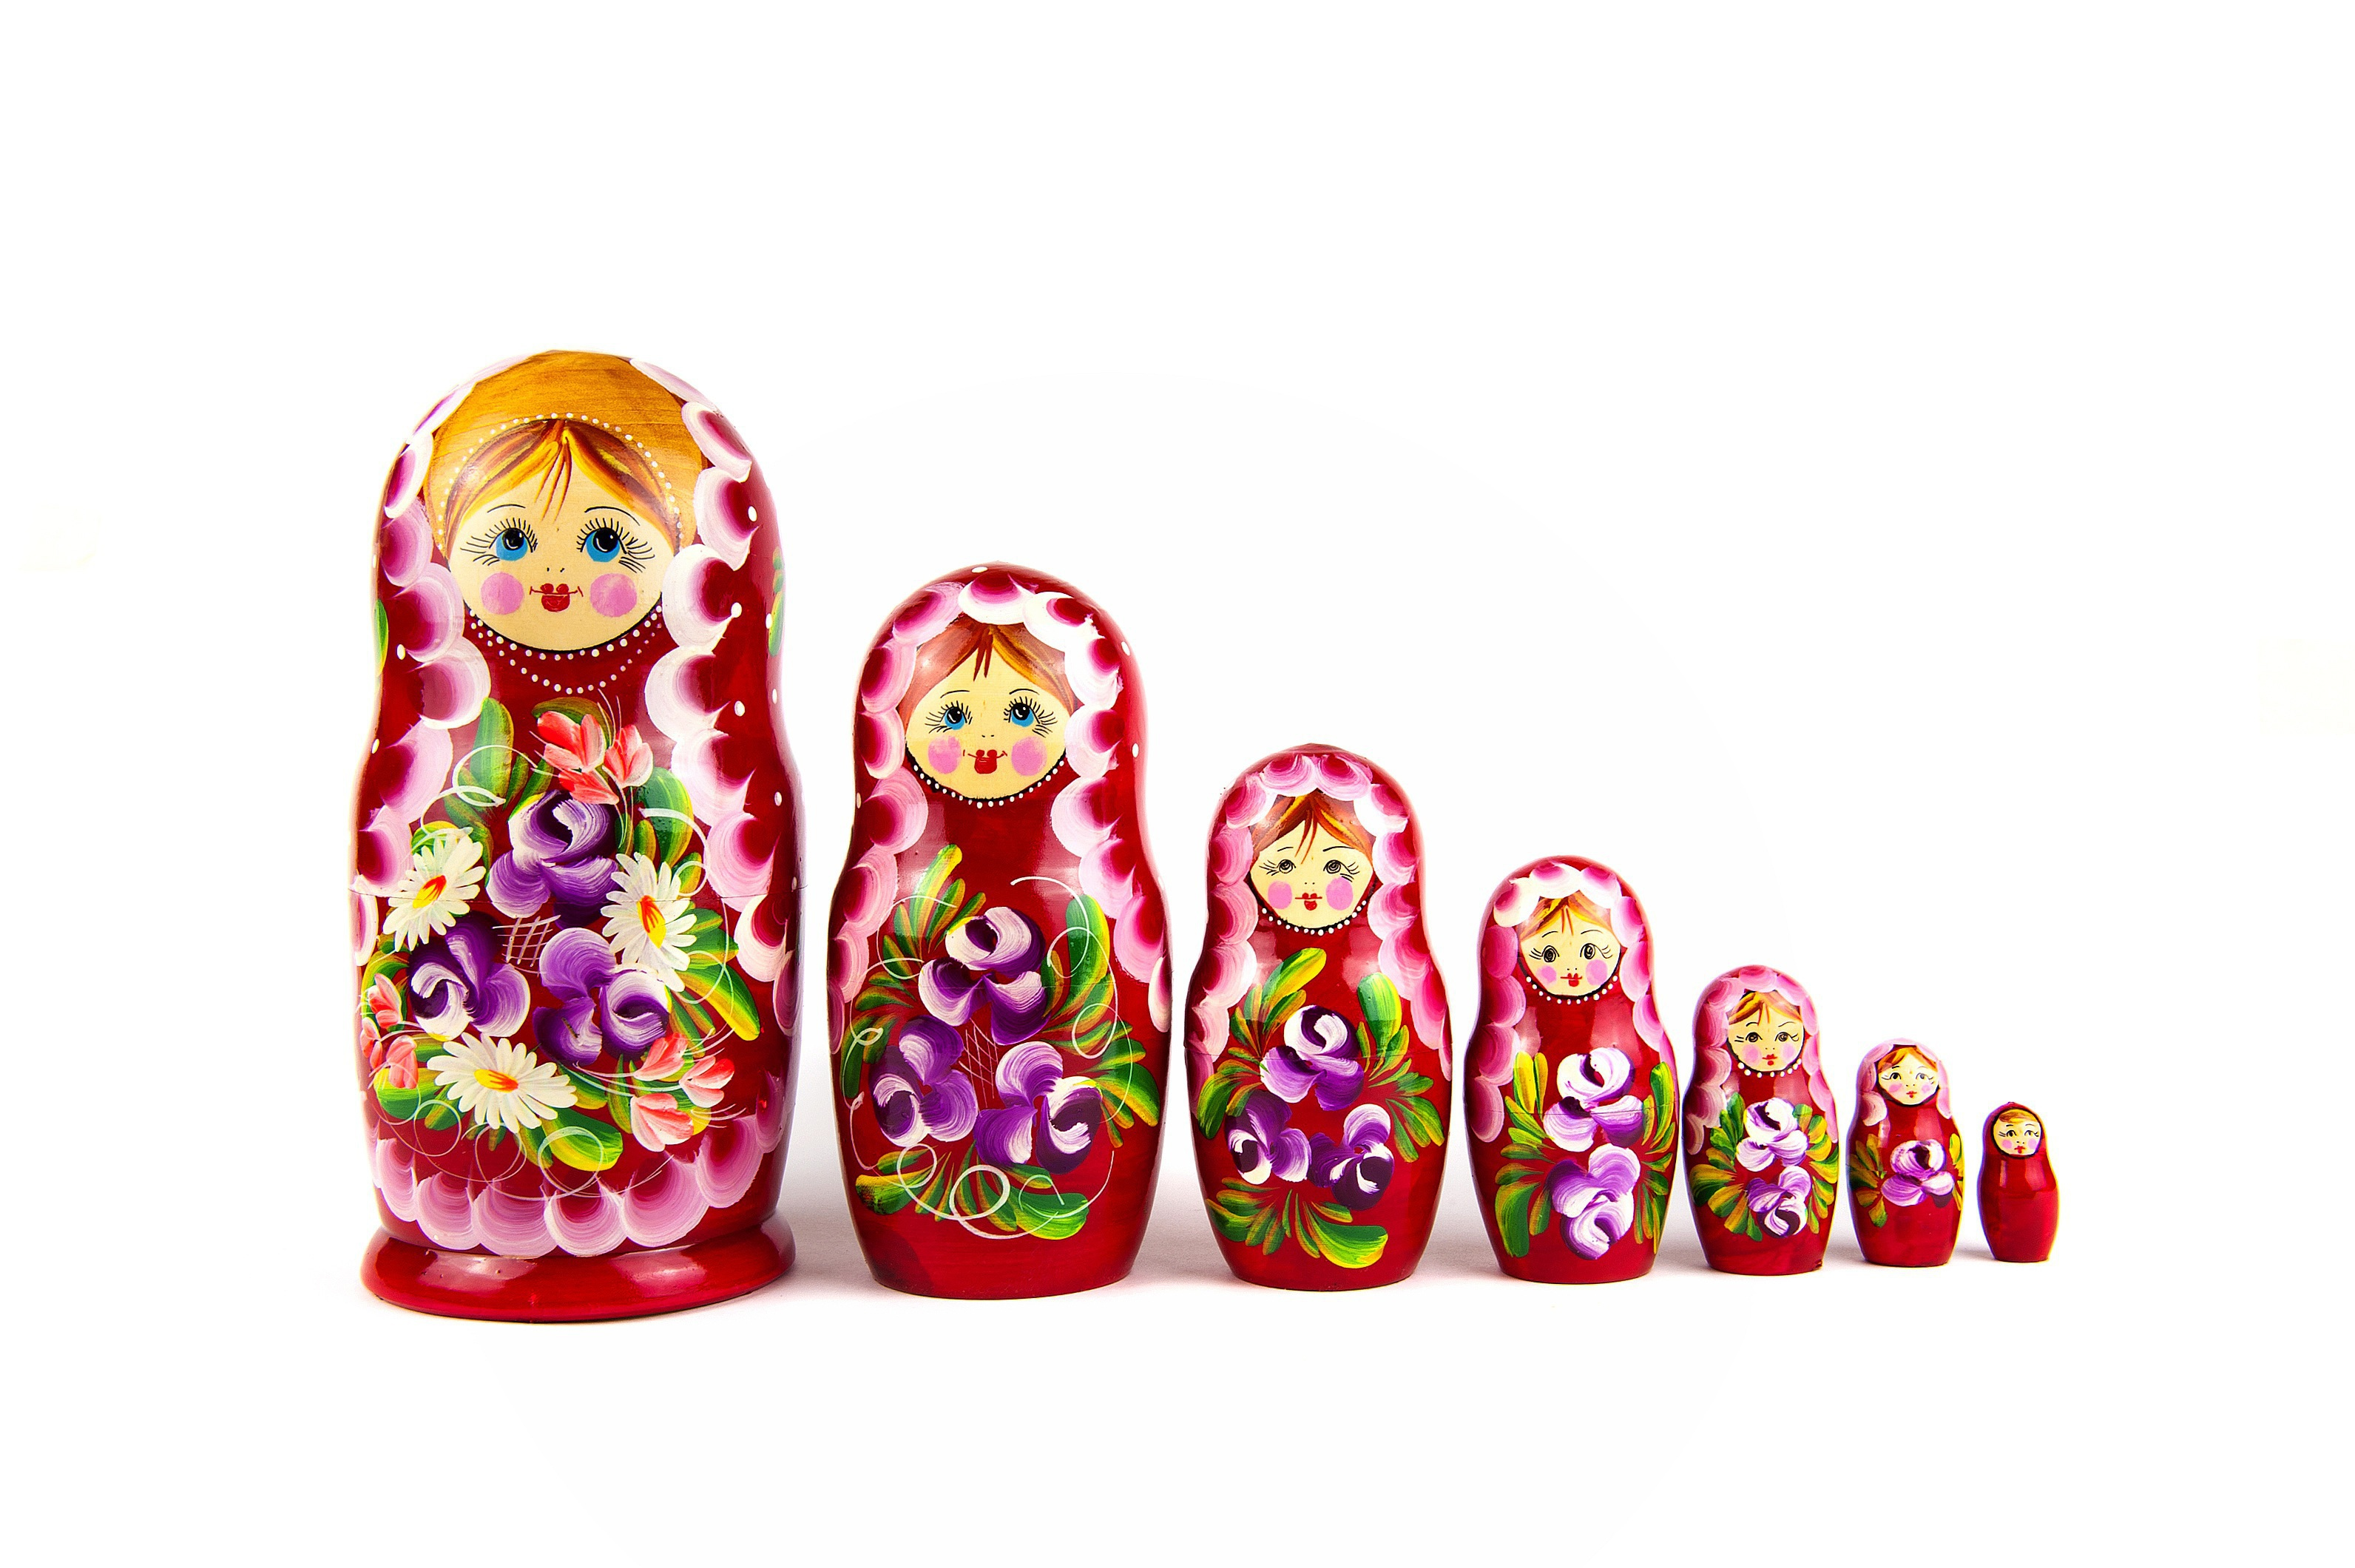
\includegraphics[keepaspectratio,width=\paperwidth]{matryoshka.jpg}}
  \begin{frame}{Recursion}
  \end{frame}
}

\begin{frame}{Back to Our Example}
  The following function counts injections:
  \[
  f(m, n) =
  \begin{cases}
    1 & \text{if } m = 0 \text{ and } n = 0 \\
    0 & \text{if } m > 0 \text{ and } n = 0 \\
    f(m, n-1) + mf(m-1, n-1) & \text{otherwise.}
  \end{cases}
  \]
  \pause
  \begin{itemize}
    \item \alert{$f(m, n)$} can be computed in \alert{$\Theta(mn)$} time
    \begin{itemize}
      \item using dynamic programming
    \end{itemize}\pause
    \item \alert{Optimal} time complexity to compute \alert{$n^{\underline{m}}$}
          is \alert{$\Theta(m)$}
    \item But \alert{$\Theta(mn)$} is still much better than translating to
          propositional logic and solving a $\#\P$-complete problem \pause
    \item The rest of this talk is about how to find such functions automatically
  \end{itemize}
\end{frame}

\begin{frame}{First-Order Knowledge Compilation: Before and After}
  \begin{columns}[b]
    \begin{column}{0.4\textwidth}
      \centering
      \begin{tikzpicture}
        \node (start) {\tiny $\forall x \in \Delta\text{. } \pP(x) \lor \qQ(x)$};
        \node[draw,rounded rectangle,fill=color2!50,below=0.7cm of start] (kc) {Compilation};
        \node[below=0.7cm of kc] (graph) {
          \scalebox{.5}{
            \begin{forest}
              for tree={sn edges,fill=red!50,ellipse,draw}
              [[
              [
              []
              []
              ]
              [
              [
              []
              []
              ]
              []
              ]
              ]]
            \end{forest}
          }
        };
        \node[draw,rounded rectangle,fill=color2!50,below=0.7cm of graph] (evaluation) {Propagation};
        \node[below=0.7cm of evaluation] (end) {
\includegraphics[height=0.4cm]{81.png}};
        \node[right=0.3cm of evaluation] (sizes) {\tiny $|\Delta| = 4$};
        \draw[-Latex,color=color2] (start) -- (kc);
        \draw[-Latex,color=color2] (kc) -- (graph);
        \draw[-Latex,color=color2] (graph) -- (evaluation);
        \draw[-Latex,color=color2] (evaluation) -- (end);
        \draw[-Latex,color=color2] (sizes) -- (evaluation);
      \end{tikzpicture}
    \end{column}
    \pause
    \begin{column}{0.6\textwidth}
      \centering
      \begin{tikzpicture}
        \node (start) {\tiny $\begin{gathered}
            \forall x \in \Gamma\text{. }\exists y \in \Delta\text{. }\pP(x, y)\\
            \forall x \in \Gamma\text{. }\forall y, z \in \Delta\text{. }\pP(x, y) \land \pP(x, z) \Rightarrow y=z\\
            \forall w, x \in \Gamma\text{. }\forall y \in \Delta\text{. }\pP(w, y) \land \pP(x, y) \Rightarrow w=x
          \end{gathered}$};
        \node[draw,rounded rectangle,fill=color2!50,below=0.3cm of start] (kc) {Compilation};
        \node[below=0.09cm of kc] (graph) {
          \scalebox{.5}{
            \begin{forest}
              for tree={sn edges,grow=0,reversed,fill=red!50}
              [,ellipse,draw,name=gdr
              [,ellipse,draw
              [,ellipse,draw
              [,ellipse,draw
              [,ellipse,draw]
              [,ellipse,draw,name=ref]
              ]
              ]
              ]
              ]
              \draw[-Latex,bend left=20] (ref) to (gdr);
            \end{forest}
          }
        };
        \node[draw,rounded rectangle,fill=color2!50,below=0.1cm of graph] (interpretation) {Conversion};
        \node[below=0.3cm of interpretation] (initial) {\tiny $f(m, n) = \sum_{l=0}^m \binom{m}{l} [l<2] \times f(m-l, n-1)$};
        \node[draw,rounded rectangle,fill=color2!50,below=0.3cm of initial] (simplification) {Simplification};
        \node[below=0.3cm of simplification] (simplified) {\tiny $f(m, n) = f(m, n-1) + mf(m-1, n-1)$};
        \node[draw,rounded rectangle,fill=color2!50,below=0.3cm of simplified] (evaluation) {Evaluation};
        \node[below=0.3cm of evaluation] (end) {
\includegraphics[height=0.4cm]{42.png}};
        \node[right=0.3cm of evaluation] (sizes) {\tiny $\begin{aligned}
                                                           f(0,0) = 1&\text{{,} }f(m, 0) = 0\\
                                                           m = 2&\text{{,} }n=7
                                                         \end{aligned}$};
        \draw[-Latex,color=color2] (start) -- (kc);
        \draw[-Latex,color=color2] (kc) -- ($(graph)+(0,0.2)$);
        \draw[-Latex,color=color2] ($(graph)+(0,-0.3)$) -- (interpretation);
        \draw[-Latex,color=color2] (interpretation) -- (initial);
        \draw[-Latex,color=color2] (initial) -- (simplification);
        \draw[-Latex,color=color2] (simplification) -- (simplified);
        \draw[-Latex,color=color2] (simplified) -- (evaluation);
        \draw[-Latex,color=color2] (evaluation) -- (end);
        \draw[-Latex,color=color2] (sizes) -- (evaluation);
      \end{tikzpicture}
    \end{column}
  \end{columns}
\end{frame}

\begin{frame}{Circuits vs Graphs}
  \begin{block}{Circuits
      \textcolor{gray}{\parencite{DBLP:conf/ijcai/BroeckTMDR11}}\ldots}
    \begin{itemize}
      \item \ldots extend d-DNNF circuits
            \textcolor{gray}{\parencite{DBLP:journals/jancl/Darwiche01}} for
            propositional knowledge compilation with \alert{more node types}
      \item \ldots are \alert{acyclic}.
    \end{itemize}
  \end{block}
  \pause
  \begin{block}{First-Order Computational Graphs (FCGs) are\ldots}
    directed \alert{\st{acyclic}} (weakly connected) graphs with:
    \begin{itemize}
    \item a single source,
    \item labelled nodes,
    \item and ordered outgoing edges.
    \end{itemize}
  \end{block}
\end{frame}

\begin{frame}{How to Interpret an FCG}
  \begin{columns}
    \begin{column}{0.25\textwidth}
      \centering
      \vspace{1cm}
      \begin{forest}
        for tree={sn edges}
        [$\GDR$,ellipse,draw,name=gdr,fill=red!50,fill on=<4>
        [$\bigvee$,ellipse,draw,name=bigvee,fill=red!50,fill on=<5>
        [$\CR$,ellipse,draw,name=cr,fill=red!50,fill on=<6>
        [$\land$,ellipse,draw,name=conj,fill=red!50,fill on=<7>
        [$\bot$,rectangle,draw,alt=<8>{fill=red!50}{fill=gray!25},name=contradiction]
        [$\Reff$,ellipse,draw,name=ref,fill=red!50,fill on=<9>]
        ]
        ]
        ]
        ]
        \draw[-Latex,bend right=45] (ref) to (gdr);
        \draw[visible on=<2-3>] (5, 42 |- gdr) node[text width=5cm,name=gdrtwo,text=color2] {\alert<3>{Generalised domain recursion}};
        \draw[visible on=<2-3>] (5, 42 |- bigvee) node[text width=5cm,name=bigveetwo,text=color2] {Deterministic set-disjunction};
        \draw[visible on=<2-3>] (5, 42 |- cr) node[text width=5cm,name=crtwo,text=color2] {\alert<3>{Constraint removal}};
        \draw[visible on=<2-3>] (5, 42 |- conj) node[text width=5cm,name=conjtwo,text=color2] {Decomposable conjunction};
        \draw[visible on=<2-3>] (5, 42 |- ref) node[text width=5cm,name=reftwo,text=color2] {\alert<3>{Caching}};
        \node[visible on=<2-3>,below=0.5cm of contradiction,name=contradictiontwo,text=color2] {Contradiction};
        \draw[visible on=<2-3>,-Latex,dashed,color=color2] (gdrtwo) -- (gdr);
        \draw[visible on=<2-3>,-Latex,dashed,color=color2] (bigveetwo) -- (bigvee);
        \draw[visible on=<2-3>,-Latex,dashed,color=color2] (crtwo) -- (cr);
        \draw[visible on=<2-3>,-Latex,dashed,color=color2] (conjtwo) -- (conj);
        \draw[visible on=<2-3>,-Latex,dashed,color=color2] (reftwo) -- (ref);
        \draw[visible on=<2-3>,-Latex,dashed,color=color2] (contradictiontwo) -- (contradiction);
      \end{forest}
    \end{column}
    \begin{column}{0.75\textwidth}
      \begin{align*}
        \onslide<4->{f(m, n) &=} \onslide<5->{\sum_{l=0}^m \binom{m}{l}} \onslide<8->{[l<2]} \onslide<7->{\times} \onslide<9->{f(m-l, n-1)}\\
        \onslide<10>{&= f(m, n-1) + mf(m-1, n-1)}
      \end{align*}
      \onslide<8>{
        \[
          [\phi] =
          \begin{cases}
            1 & \text{if } \phi \\
            0 & \text{if } \neg\phi
          \end{cases}
          \]
      }
    \end{column}
  \end{columns}
\end{frame}

\begin{frame}{Compilation: How FCGs Are Built}
  \begin{definition}
    A \alert{(compilation) rule} is a function that takes a \alert{formula} and returns a set of \alert{$(G, L)$} pairs, where
    \begin{itemize}
    \item \alert{$G$} is an FCG,
    \item and \alert{$L$} is a list of formulas.
    \end{itemize}
  \end{definition}
  \vfill The formulas in \alert{$L$} are then \alert{compiled}, and the
  resulting FCGs are \alert{inserted} into \alert{$G$} according to a \alert{set
    order}.
\end{frame}

\begin{frame}{Example Compilation Rule: Independence}
  Input formula:
  \begin{gather}
    ({\color{color1} \forall x, y \in \Omega\text{. }x=y}) \land \label{eq:1} \tag{{\color{color1} 1}} \\
    ({\color{color2} \forall x \in \Gamma\text{. }\forall y, z \in \Delta\text{. }\texttt{P}(x, y) \land \texttt{P}(x, z) \Rightarrow y=z}) \land \label{eq:2} \tag{{\color{color2} 2}} \\
    ({\color{color2} \forall w, x \in \Gamma\text{. }\forall y \in \Delta\text{. }\texttt{P}(w, y) \land \texttt{P}(x, y) \Rightarrow w=x}) \label{eq:3} \tag{{\color{color2} 3}}
  \end{gather}
  \pause
  Only one \alert{(G, L)} pair:
  \[
  G =
  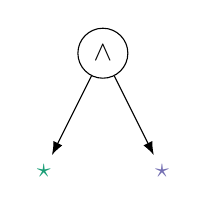
\begin{tikzpicture}[edge from parent/.style={draw,-Latex},baseline=(current bounding box.center)]
    \node[draw,circle] {$\land$}
    child {node {\color{color1} $\star$}}
    child {node {\color{color2} $\star$}}
    ;
  \end{tikzpicture},
  \qquad
  L = \langle {\color{color1} \eqref{eq:1}}, {\color{color2} \eqref{eq:2} \land \eqref{eq:3}} \rangle
  \]
\end{frame}
% stars mark edges to nowhere and they are associated with the formulas in L via a certain order

\begin{frame}
  \frametitle<1>{New Rule 1/3: Generalised Domain Recursion}
  \frametitle<2>{New Rule 2/3: Constraint Removal}
  \frametitle<3>{New Rule 3/3: Identifying Possibilities for Recursion}
  \begin{columns}
    \begin{column}{0.15\textwidth}
      \centering
      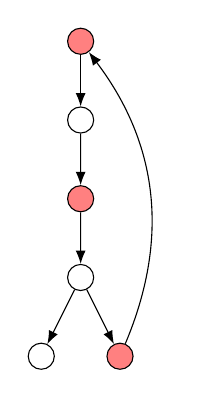
\begin{tikzpicture}[every node/.style={draw,ellipse},edge from parent/.style={draw,-Latex},sibling distance=10mm,level distance=10mm]
        \node[fill=red!50, fill on=<1>] (dr) {}
        child {node {}
          child {node[fill=red!50, fill on=<2>] {}
            child {node {}
              child {node {}}
              child {node[fill=red!50, fill on=<3>] (ref) {}}
            }}};
        \draw[-Latex, bend right,alt=<3>{red}{black}] (ref) to (dr);
      \end{tikzpicture}
    \end{column}
    \begin{column}{0.85\textwidth}
      \begin{overprint}
        \onslide<1>
          \begin{example}
            Input formula:
            \[
              \forall x \in \Gamma\text{. }\forall y, z \in \Delta\text{. }y \ne z \Rightarrow \neg \texttt{P}(x, y) \lor \neg \texttt{P}(x, z)
            \]
            Output formula (with a new constant \alert{$c \in \Gamma$}):
            \begin{gather*}
              \forall y, z \in \Delta\text{. }y \ne z \Rightarrow \neg \texttt{P}(\alert{c}, y) \lor \neg \texttt{P}(\alert{c}, z) \\
              \begin{multlined}
                \forall x \in \Gamma\text{. }\forall y, z \in \Delta\text{. }\alert{x \ne c} \land y \ne z \Rightarrow \\
                \neg \texttt{P}(x, y) \lor \neg \texttt{P}(x, z)
              \end{multlined}
            \end{gather*}
            %% Output FCG:
            %% \begin{tikzpicture}[edge from parent/.style={draw,-latex}]
            %%   \node[draw,circle] {$\textsc{DR}$}
            %%   child {node {$\star$}}
            %%   ;
            %% \end{tikzpicture}
          \end{example}
        \onslide<2>
          \begin{example}
            Input formula (with a constant \alert{$c \in \Gamma$}):
            \begin{gather*}
              \begin{multlined}
                \forall x \in \alert{\Gamma}\text{. }\forall y, z \in \Delta\text{. }\alert{x \ne c} \land y \ne z \Rightarrow \\
                \neg \texttt{P}(x, y) \lor \neg \texttt{P}(x, z)
              \end{multlined} \\
              \begin{multlined}
                \forall w,x \in \alert{\Gamma}\text{. }\forall y \in \Delta\text{. }\alert{w \ne c} \land \alert{x \ne c} \land w \ne x \Rightarrow \\
                \neg \texttt{P}(w, y) \lor \neg \texttt{P}(x, y)
              \end{multlined}
            \end{gather*}
            Output formula (with a new domain \alert{$\Gamma' \coloneqq \Gamma \setminus \{\, c \,\}$}):
            \begin{gather*}
              \forall x \in \alert{\Gamma'}\text{. }\forall y, z \in \Delta\text{. }y \ne z \Rightarrow \neg \texttt{P}(x, y) \lor \neg \texttt{P}(x, z) \\
              \forall w,x \in \alert{\Gamma'}\text{. }\forall y \in \Delta\text{. }w \ne x \Rightarrow \neg \texttt{P}(w, y) \lor \neg \texttt{P}(x, y)
            \end{gather*}
          \end{example}
        \onslide<3>
          \begin{block}{Goal}
            Check if the input formula is equivalent (up to domains) to a
            previously encountered formula.
          \end{block}
          \begin{block}{Outline}
            \begin{enumerate}
              \item Consider pairs of `similar' clauses.
              \item Consider bijections between their sets of variables.
              \item Extend each such bijection to a map between sets of domains.
              \item If the bijection makes the clauses equal, and the domain map
                    is compatible with previous domain maps, move on to another
                    pair of clauses.
            \end{enumerate}
          \end{block}
      \end{overprint}
    \end{column}
  \end{columns}
\end{frame}

% an example on partial injection (i.e., bipartite matching) counting
\begin{frame}{How These Rules Fit Together (1/5)}
  \begin{tikzpicture}[overlay,remember picture]
    \node[draw,rounded rectangle,fill=color2!50,anchor=center,above=0.5cm] at (current page.center) (rules) {Generalised domain recursion};
    \node[above=of rules] (before) {$\begin{gathered}
        \forall x \in \alert{\Gamma}\text{. }\forall y, z \in \Delta\text{. }y \ne z \Rightarrow \neg\pP(x, y) \lor \neg\pP(x, z)\\
        \forall w,x \in \alert{\Gamma}\text{. }\forall y \in \Delta\text{. }w \ne x \Rightarrow \neg\pP(w, y) \lor \neg\pP(x, y)
      \end{gathered}$};
    \node[below=of rules] (after) {$\begin{gathered}
        \forall y, z \in \Delta\text{. }y \ne z \Rightarrow \neg\pP(\alert{c}, y) \lor \neg\pP(\alert{c}, z)\\
        \forall x \in \Gamma\text{. }\forall y,z \in \Delta\text{. }y \ne z \land \alert{x \ne c} \Rightarrow \neg\pP(x, y) \lor \neg\pP(x, z)\\
        \forall x \in \Gamma\text{. }\forall y \in \Delta\text{. }\alert{x \ne c} \Rightarrow \neg\pP(\alert{c}, y) \lor \neg\pP(x, y)\\
        \forall w \in \Gamma\text{. }\forall y \in \Delta\text{. }\alert{w \ne c} \Rightarrow \neg\pP(w, y) \lor \neg\pP(\alert{c}, y)\\
        \forall w,x \in \Gamma\text{. }\forall y \in \Delta\text{. }w \ne x \land \alert{w \ne c} \land \alert{x \ne c} \Rightarrow \neg\pP(w, y) \lor \neg\pP(x, y)
      \end{gathered}$};
    \begin{scope}[on background layer]
      \node[anchor=north,fill=greenish,minimum width=11.1cm,minimum height=0.7cm] at (before.north) {};
      \node[anchor=south,fill=blueish,minimum width=11.1cm,minimum height=0.7cm] at (before.south) {};
      \node[anchor=north,fill=greenish,minimum width=11.1cm,minimum height=1.3cm] at (after.north) {};
      \node[anchor=south,fill=blueish,minimum width=11.1cm,minimum height=2cm] at (after.south) {};
    \end{scope}
    \draw[-Latex,color=color2,ultra thick,shorten <=0.1cm,shorten >=0.1cm] (before) -- (rules);
    \draw[-Latex,color=color2,ultra thick,shorten <=0.1cm,shorten >=0.1cm] (rules) -- (after);
  \end{tikzpicture}
\end{frame}

\begin{frame}{How These Rules Fit Together (2/5)}
  \begin{tikzpicture}[overlay,remember picture]
    \node[draw,rounded rectangle,fill=color2!50,anchor=center,below=1cm] at (current page.center) (rules) {Atom counting and unit propagation};
    \node[above=of rules] (before) {$\begin{gathered}
        \forall y, z \in \Delta\text{. }y \ne z \Rightarrow \neg\pP(\alert{c}, y) \lor \neg\pP(\alert{c}, z)\\
        \forall x \in \Gamma\text{. }\forall y,z \in \Delta\text{. }y \ne z \land \alert{x \ne c} \Rightarrow \neg\pP(x, y) \lor \neg\pP(x, z)\\
        \forall x \in \Gamma\text{. }\forall y \in \Delta\text{. }\alert{x \ne c} \Rightarrow \neg\pP(\alert{c}, y) \lor \neg\pP(x, y)\\
        \forall w \in \Gamma\text{. }\forall y \in \Delta\text{. }\alert{w \ne c} \Rightarrow \neg\pP(w, y) \lor \neg\pP(\alert{c}, y)\\
        \forall w,x \in \Gamma\text{. }\forall y \in \Delta\text{. }w \ne x \land \alert{w \ne c} \land \alert{x \ne c} \Rightarrow \neg\pP(w, y) \lor \neg\pP(x, y)
      \end{gathered}$};
    \node[below=of rules] (after) {$\begin{gathered}
        \forall y, z \in \alert{\Delta^{\top}}\text{. }y \ne z \Rightarrow \bot\\
        \forall x \in \Gamma\text{. }\forall y, z \in \alert{\Delta^{\bot}}\text{. }y \ne z \land x \ne c \Rightarrow \neg\pP(x, y) \lor \neg\pP(x, z) \\
        \forall w, x \in \Gamma\text{. }\forall y \in \alert{\Delta^{\bot}}\text{. }w \ne x \land w \ne c \land x \ne c \Rightarrow \neg\pP(w, y) \lor \neg\pP(x, y)
      \end{gathered}$};
    \draw[-Latex,color=color2,ultra thick,shorten <=0.1cm,shorten >=0.1cm] (before) -- (rules);
    \draw[-Latex,color=color2,ultra thick,shorten <=0.1cm,shorten >=0.1cm] (rules) -- (after);
    \draw[-Latex,color=color2,ultra thick,shorten <=0.1cm,shorten >=0.1cm] (rules) -- (after);
  \end{tikzpicture}
\end{frame}

\begin{frame}{How These Rules Fit Together (3/5)}
  \begin{tikzpicture}[overlay,remember picture]
    \node[draw,rounded rectangle,fill=color2!50,anchor=center] at (current page.center) (rules) {Constraint removal};
    \node[above=of rules] (before) {$\begin{gathered}
        \forall y, z \in \Delta^{\top}\text{. }y \ne z \Rightarrow \bot\\
        \forall x \in \alert{\Gamma}\text{. }\forall y, z \in \Delta^{\bot}\text{. }y \ne z \land \alert{x \ne c} \Rightarrow \neg\pP(x, y) \lor \neg\pP(x, z) \\
        \forall w, x \in \alert{\Gamma}\text{. }\forall y \in \Delta^{\bot}\text{. }w \ne x \land \alert{w \ne c} \land \alert{x \ne c} \Rightarrow \neg\pP(w, y) \lor \neg\pP(x, y)
      \end{gathered}$};
    \node[below=of rules] (after) {$\begin{gathered}
        \forall y, z \in \Delta^{\top}\text{. }y \ne z \Rightarrow \bot\\
        \forall x \in \alert{\Gamma'}\text{. }\forall y, z \in \Delta^{\bot}\text{. }y \ne z \Rightarrow \neg\pP(x, y) \lor \neg\pP(x, z) \\
        \forall w, x \in \alert{\Gamma'}\text{. }\forall y \in \Delta^{\bot}\text{. }w \ne x \Rightarrow \neg\pP(w, y) \lor \neg\pP(x, y)
      \end{gathered}$};
    \draw[-Latex,color=color2,ultra thick,shorten <=0.1cm,shorten >=0.1cm] (before) -- (rules);
    \draw[-Latex,color=color2,ultra thick,shorten <=0.1cm,shorten >=0.1cm] (rules) -- (after);
  \end{tikzpicture}
\end{frame}

\begin{frame}{How These Rules Fit Together (4/5)}
  \begin{tikzpicture}[overlay,remember picture]
    \node[draw,rounded rectangle,fill=color2!50,anchor=center] at (current page.center) (rules) {Independence};
    \node[above=of rules] (before) {$\begin{gathered}
        \forall y, z \in \alert{\Delta^{\top}}\text{. }y \ne z \Rightarrow \bot\\
        \forall x \in \alert{\Gamma'}\text{. }\forall y, z \in \alert{\Delta^{\bot}}\text{. }y \ne z \Rightarrow \neg\pP(x, y) \lor \neg\pP(x, z) \\
        \forall w, x \in \alert{\Gamma'}\text{. }\forall y \in \alert{\Delta^{\bot}}\text{. }w \ne x \Rightarrow \neg\pP(w, y) \lor \neg\pP(x, y)
      \end{gathered}$};
    \node[below left=of rules,fill=greenish] (after1) {$\forall y, z \in \alert{\Delta^{\top}}\text{. }y \ne z \Rightarrow \bot$};
    \node[below right=2cm and -4cm of rules,fill=blueish] (after2) {$\begin{gathered}
        \forall x \in \alert{\Gamma'}\text{. }\forall y, z \in \alert{\Delta^{\bot}}\text{. }y \ne z \Rightarrow \neg\pP(x, y) \lor \neg\pP(x, z) \\
        \forall w, x \in \alert{\Gamma'}\text{. }\forall y \in \alert{\Delta^{\bot}}\text{. }w \ne x \Rightarrow \neg\pP(w, y) \lor \neg\pP(x, y)
      \end{gathered}$};
    \begin{scope}[on background layer]
      \node[anchor=north,fill=greenish,minimum width=9cm,minimum height=0.7cm] at (before.north) {};
      \node[anchor=south,fill=blueish,minimum width=9cm,minimum height=1.3cm] at (before.south) {};
    \end{scope}
    \draw[-Latex,color=color2,ultra thick,shorten <=0.1cm,shorten >=0.1cm] (before) -- (rules);
    \draw[-Latex,color=color2,ultra thick,shorten <=0.1cm,shorten >=0.1cm] (rules) -- (after1);
    \draw[-Latex,color=color2,ultra thick,shorten <=0.1cm,shorten >=0.1cm] (rules) -- (after2);
  \end{tikzpicture}
\end{frame}

\begin{frame}{How These Rules Fit Together (5/5): Recursion}
  \centering
  \begin{tikzpicture}[overlay,remember picture]
    \node[anchor=center,above=0.5cm] at (current page.center) (equal) {\rotatebox{90}{\textcolor{color2}{\Huge$=$}}};
    \node[below=0.5cm of equal] (after1) {$\begin{gathered}
        \forall x \in \alert{\Gamma}\text{. }\forall y, z \in \alert{\Delta}\text{. }y \ne z \Rightarrow \neg\pP(x, y) \lor \neg\pP(x, z)\\
        \forall w,x \in \alert{\Gamma}\text{. }\forall y \in \alert{\Delta}\text{. }w \ne x \Rightarrow \neg\pP(w, y) \lor \neg\pP(x, y)
      \end{gathered}$};
    \node[above=0.5cm of equal] (foo) {$\begin{gathered}
        \forall x \in \alert{\Gamma'}\text{. }\forall y, z \in \alert{\Delta^{\bot}}\text{. }y \ne z \Rightarrow \neg\pP(x, y) \lor \neg\pP(x, z) \\
        \forall w, x \in \alert{\Gamma'}\text{. }\forall y \in \alert{\Delta^{\bot}}\text{. }w \ne x \Rightarrow \neg\pP(w, y) \lor \neg\pP(x, y)
      \end{gathered}$};
    \node[below=0.5cm of after1] (plus) {\textcolor{color2}{\Huge$+$}};
    \node[below=0.5cm of plus] {$\{\, \alert{\Gamma} \mapsto \alert{\Gamma'}, \alert{\Delta^{\bot}} \mapsto \alert{\Delta} \,\}$};
  \end{tikzpicture}
\end{frame}

%% \begin{frame}{Compilation as Search}
%%   \begin{definition}
%%     A \alert{(search) state} is a tuple \structure{$(G, C, L)$}, where:
%%     \begin{itemize}
%%     \item \structure{$G$} is an FCG (or \texttt{null}),
%%     \item \structure{$C$} is a compilation cache that maps integers to sets of pairs $(\phi, v)$, where $\phi$ is a formula, and $v$ is a node of $G$ (which is used to identify opportunities for recursion),
%%     \item and \structure{$L$} is a list of formulas (that are yet to be compiled). (Note that the order is crucial!)
%%     \end{itemize}
%%   \end{definition}
%%   The search algorithm combines greedy and breadth-first search:
%% \end{frame}

\begin{frame}{Resulting Improvements to Counting Functions}
  Let \alert{$\Gamma$} and \alert{$\Delta$} be two sets with
  cardinalities \alert{$|\Gamma| = m$} and \alert{$|\Delta| = n$}.

  Our new rules enable Crane to efficiently count
  \alert{$\Gamma \to \Delta$} functions such as:
  \begin{itemize}
    \item injections in \alert{$\Theta(mn)$} time
          \begin{itemize}
            \item by hand: \alert{$\Theta(m)$}
          \end{itemize}
    \item partial injections in \alert{$\Theta(mn)$} time
          \begin{itemize}
            \item by hand: \alert{$\Theta({\min\{\, m, n \,\}}^2)$}
          \end{itemize}
          \item bijections in \alert{$\Theta(m)$} time
          \begin{itemize}
            \item \alert{optimal!}
            \item FastWFOMC seems to be \alert{$\Omega(m^{4})$}
          \end{itemize}
  \end{itemize}
\end{frame}
% TODO: add 2 more statements about fastwfomc, showing their plots on the RHS
% when revealing them

{ % all template changes are local to this group.
    \setbeamertemplate{navigation symbols}{}
    \begin{frame}<article:0>[plain]
        \begin{tikzpicture}[remember picture,overlay]
            \node[at=(current page.center)] {
                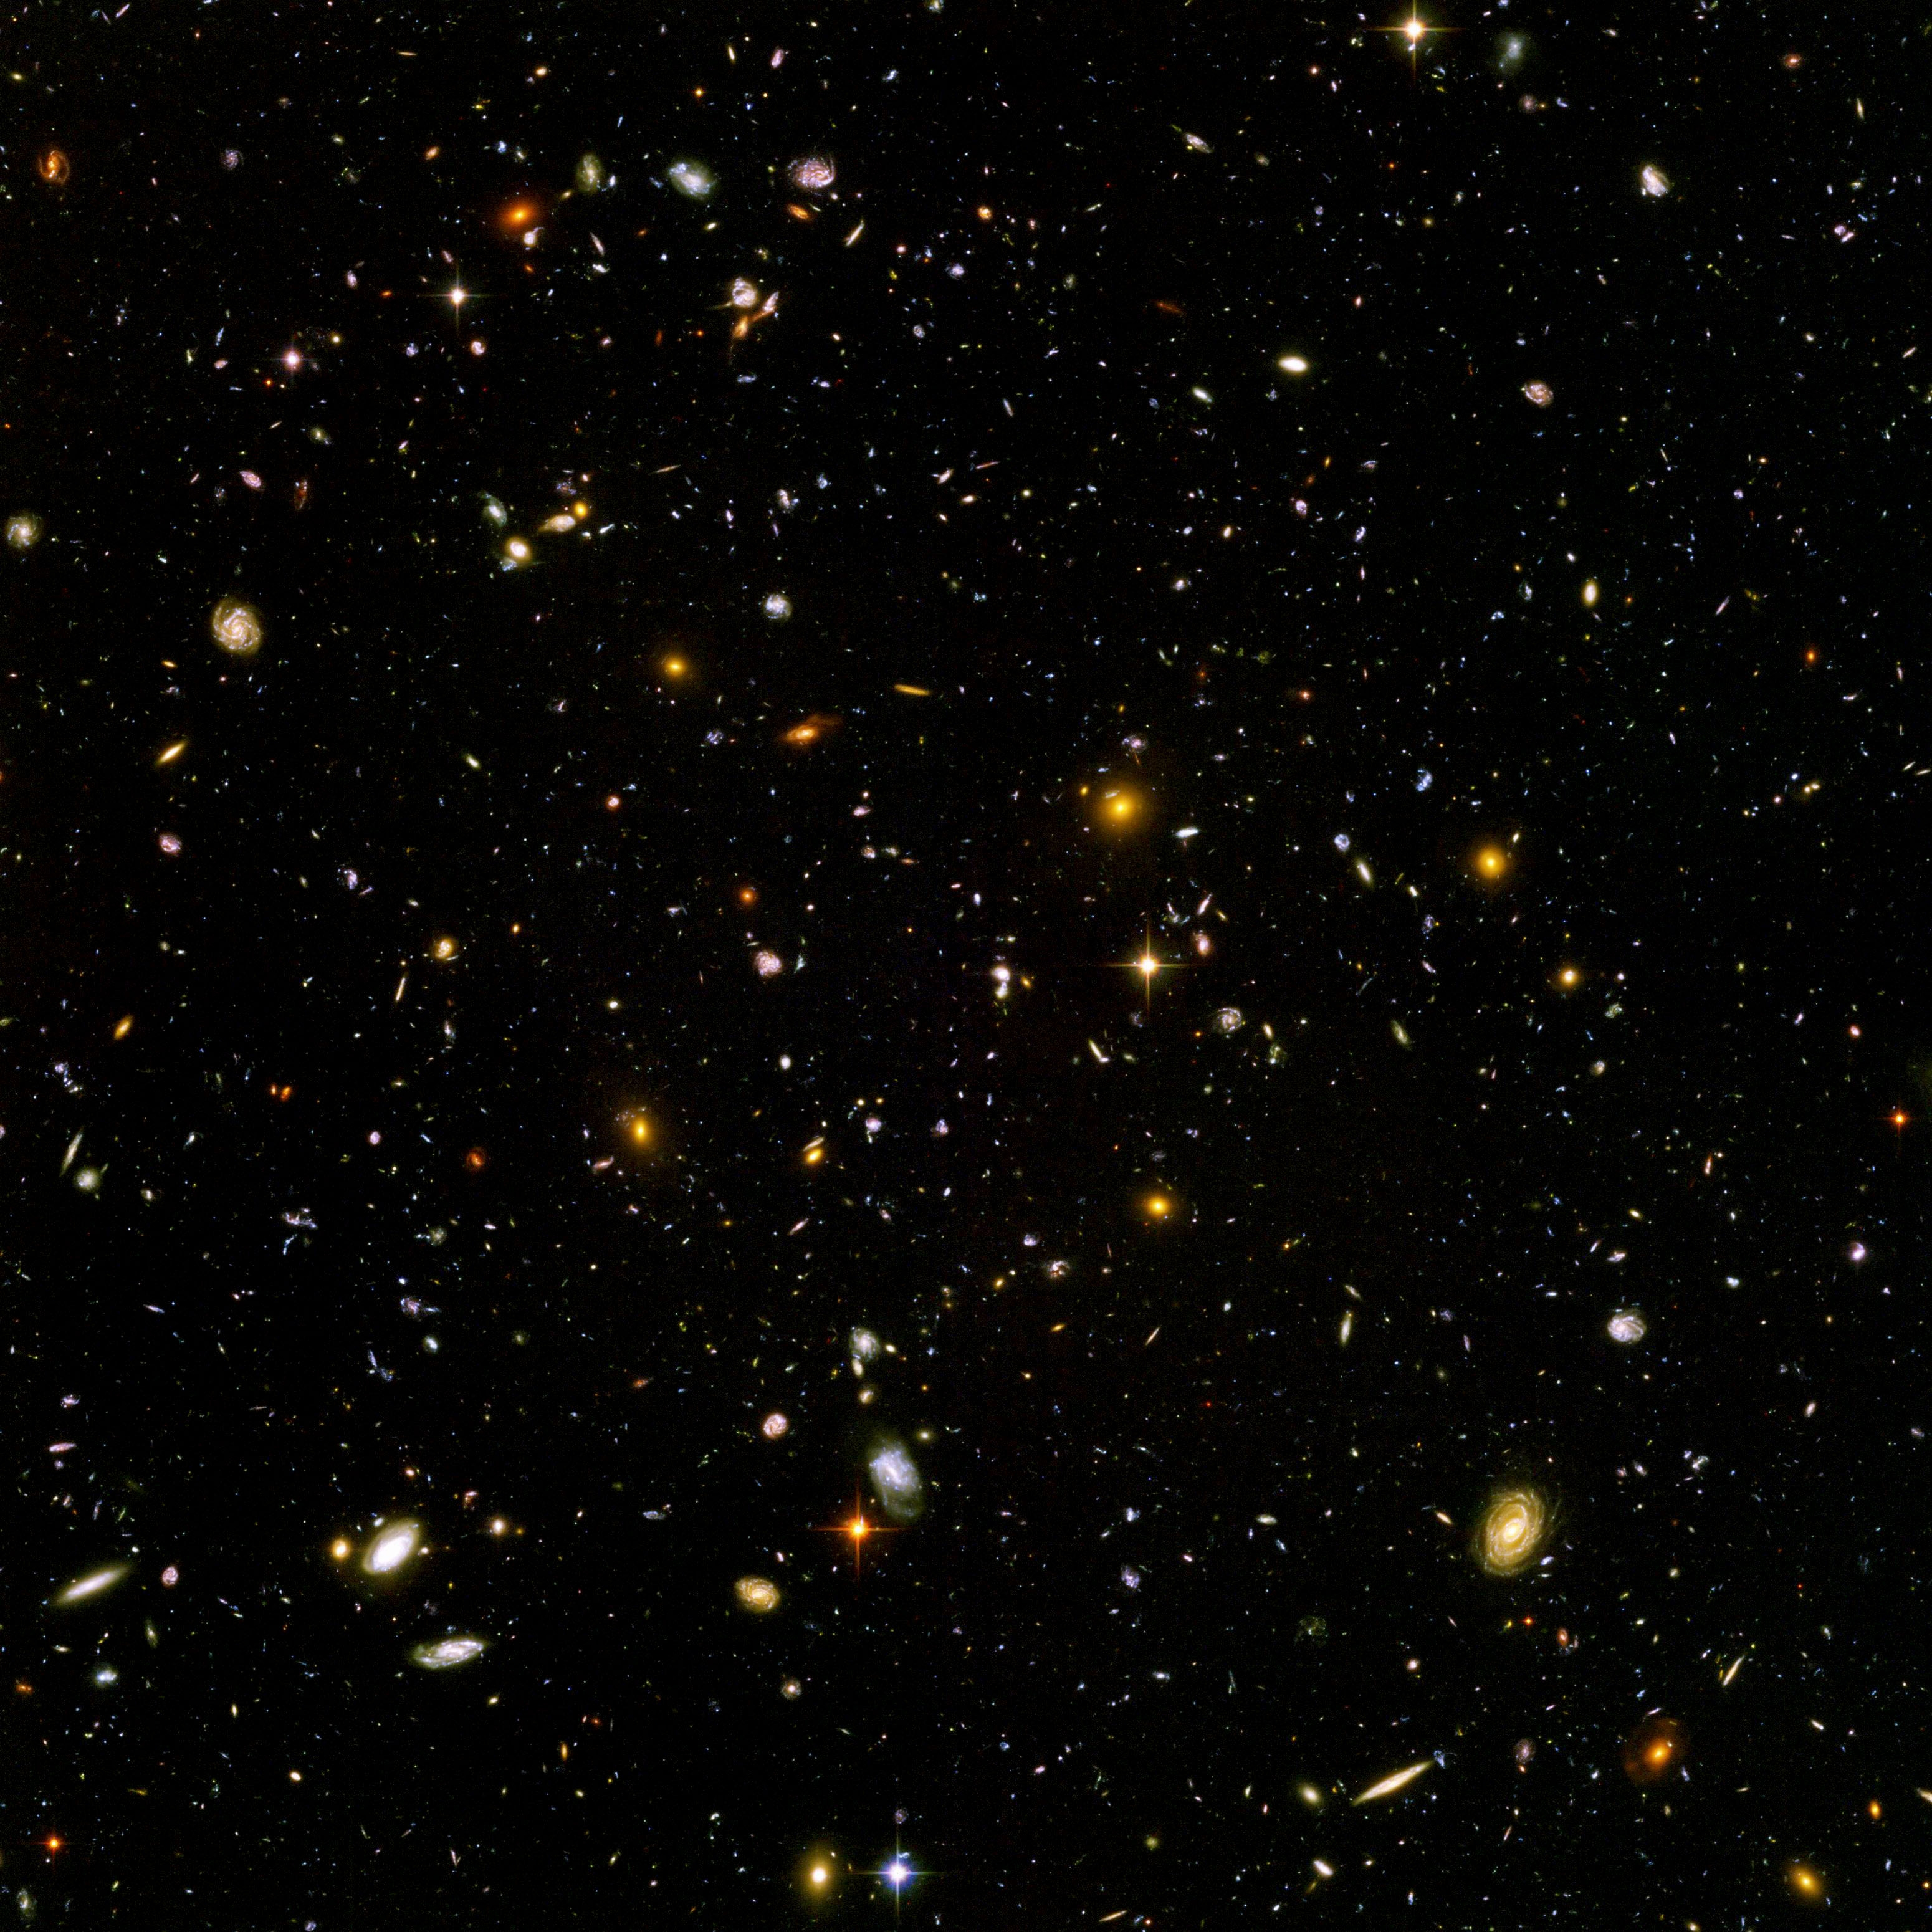
\includegraphics[keepaspectratio, width=\paperwidth]{hubble.jpg}
            };
            \node[shift=({-0.7, 0.1})] at (current page.south east) {\tiny \textcolor{lightgray}{Source: NASA}};
        \end{tikzpicture}
     \end{frame}
}

% TODO: need 3 slides in total for the ending

% really focus on the 'so what?'
\begin{frame}{Summary \& Future Work}
  \begin{block}{Summary}
    The circuits hitherto used for FOMC become more powerful with:
    \begin{itemize}
    \item cycles,
    \item generalised domain recursion,
    \item and some more new compilation rules that support domain recursion.
    \end{itemize}
  \end{block}
  \begin{block}{Future Work}
    \begin{itemize}
    \item Automate:
      \begin{itemize}
      \item extracting and simplifying the definitions of functions,
      \item finding all base cases.
      \end{itemize}
    \item Open questions:
      \begin{itemize}
      \item What kind of \alert{sequences} are computable in this way?
      \item Would using a \alert{different logic} extend the capabilities of FOMC further?
      \end{itemize}
    \end{itemize}
  \end{block}
\end{frame}

\begin{frame}{Major Directions for Future Work}
  \begin{itemize}
    \item An algebraic description of what kind of sequences and functions with
          domain $\mathbb{N}_{0}^{k}$ are computable in this way
          \begin{itemize}
            \item monotonicity, maximal growth rate, etc.
          \end{itemize}
    \item A different input format or logic that allows the same approach to
          capture more computations
          \begin{itemize} % TODO: come back to the 'many ways to count' slide
                          % and add more arrows (e.g., beyond FOL)
            \item fixed-point logic with counting
            \item `let domain $\Delta \coloneqq \{\, 1, 2, \dots, MC(\phi) \,\}$'
          \end{itemize}
    \item parameterised Markov logic networks
    \begin{itemize}
      \item `What equations do the domain sizes have to satisfy for the
            probability of event $E$ to be at least $95\%$?'
    \end{itemize}
  \end{itemize}
\end{frame}

\end{document}
